\chapter{Physics Fundamentals}\label{chap:fundamentals}
The section \ref{sec:measurement} establishes a short overview of the physical quantities relevant to be measured by the instruments in order to determine power consumption. Section \ref{sec:vflux} introduces the considerations of noise encountered during measurement due to voltage fluctuations. 
\section{Physical quantities}\label{sec:measurement}
To establish a robust data basis, a compressed investigation on the physical fundamentals has to be made, in order to ensure a realistic expectation on the available data can be expected.
Instantaneous electrical power (P) is defined as the derivative of electrical energy over at time $t_{0}$. Electrical energy (W) is the combination of the electric current (I), defined as transported charge (Q) over time, and the electric voltage (V) of electric particles moving in an electric circuit/cite{Hacker2020}. Given the measurement of each quantity is determined as the average value over a measurement interval, all quantities are also defined as constant over the given time period. Therefore the relevant electric properties of the system can be described by the simplified formula shown in equation \ref{eq:electric formula}. 
\begin{equation}
	W = P \times t = I\times V \times t = V \times Q
	\label{eq:electric formula}
\end{equation}
By observation of the formula, the act of measuring the amount of power consumed in an electrical system is accomplished by determining the electrical potential and electrical current in a system over a given amount of time.

\section{Voltage Fluctuations}\label{sec:vflux}
The first component of interest is the voltage provided by the outlets used in IT application environments. In European countries, the amount and fluctuations of the electric grid is regulated in European standard '\gls{EN} (EN) 50160'.
By this standardization boundaries on frequency, voltage fluctuation, flickering, faults and other quantities were given. As most regulations regard the quality and safety of the power grid, an overview on relevant standards for measurement needs is given in table \ref{tab:en50160}. Due to the given voltage fluctuation ranges, a theoretical measurement error of 10\% could be expected on instantaneous measurements, due to noise in the mean voltage value of 230V.  As quality standards also demand the fluctuations to be ideally symmetrical, noise in the voltage supplied should mostly cancel out when averaging over multiple measurements.
For this reason, a method with a sufficient surplus of separate measurements, averaged over a larger time span, should be considered preferable. In this thesis, the fluctuations in measurement due to voltage issues is considered negligible.

\begin{table}[ht]
	\centering
	\begin{tabular}{|c|c|}
		\hline
		frequency & 50 Hz (+/- 1\%) \\
		\hline
		voltage fluctuation (slow) & 230 V (+/- 10\%) \\
		\hline
		voltage fluctuation (fast) & 230 V (+/- 5\%) \\
		\hline
		voltage faults (short) & < 1000 per year\\
		\hline
		voltage faults (long) & < 50 per year\\
		\hline
	\end{tabular}
	\caption{extract of standardization values given in EN 50160 \cite{EN50160}.}
	\label{tab:en50160}
\end{table}

\section{Determining Electric Current}\label{sec:current}
By analyzing the electric formula of equation \ref{eq:electric formula} and the conclusion of section \ref{sec:vflux} the power measurement is directly correlated to the electrical current an office appliance is drawing from the grid. In electrical engineering, different methods to determine the current in an electric circuit are known. The most direct way would consist of a separately closed electric circuit where voltage drops on a standardized resistor. However, this approach does not allow the observation of an already established supply system. The application of measuring 'in-use' appliances, requires different methods, like the usage linear current hall effect sensors.

\subsubsection{Hall Effect}
The hall effect is a physical phenomenon, named after US physicist Edwin Hall: 1855 – 1938. The effect "...occurs in a current-carrying conductor
that is located in a magnetic field. Thereby an electric field builds up which is perpendicular to the current direction and the magnetic field and compensates the Lorentz force affecting the electrons" \cite{Hacker2020_Hall}.
In figure \ref{fig:hall_sensor_block} a depiction of the hall sensor and its components can be viewed. Basically the conducting sheet measures a permeating magnetic field 'H' by the voltage differential '$V_H$' created through Lorentz forces (F$_L$) affecting the 'Constant Current Flow'. This is possible, as the hall voltage is rising, until its equivalent electric force (F$_e$) creates an equilibrium. The electric field strength (E) is equivalent to the hall voltage (V$_H$) divided by the diameter of the conductor plate (d)The strength the Lorentz force is directly proportional to the strength of the magnetic field (B), as well as drift velocity (v) and charge (q) of the current. The drift velocity of the particles is dictated by the current and cross section of the conductor. All relevant quantities can be computed using formula \ref{eq:hall_formula}.
\begin{equation}
	F_e = E \times q = \frac{V_H}{d} \times q =  B \times v \times q = F_L
	\label{eq:hall_formula}
\end{equation}
Rearranged the strength of the directional magnetic field is computed as shown in equation \ref{eq:hall_formula_rearranged}.
\begin{equation}
	B = \dfrac{V_H}{d \times v}
	\label{eq:hall_formula_rearranged}
\end{equation}
As every flowing current induces an electromagnetic field around the conduction it is traversing, the hall effect can be utilized to directly measure the current of a nearby electric circuit. Depending on the design of the sensor unit, the direction of electric current (positive or negative) can be distinguished. With additional amplification, trim settings and filtering, a clearer signal can be deduced, as alternating current does not produce a constant electromagnetic field. These sensors often are designated as linear current hall effect sensors. A simplified block diagram of such a hall sensor can be seen in figure \ref{fig:lcs_block}
\begin{figure}[th]
	\centering
	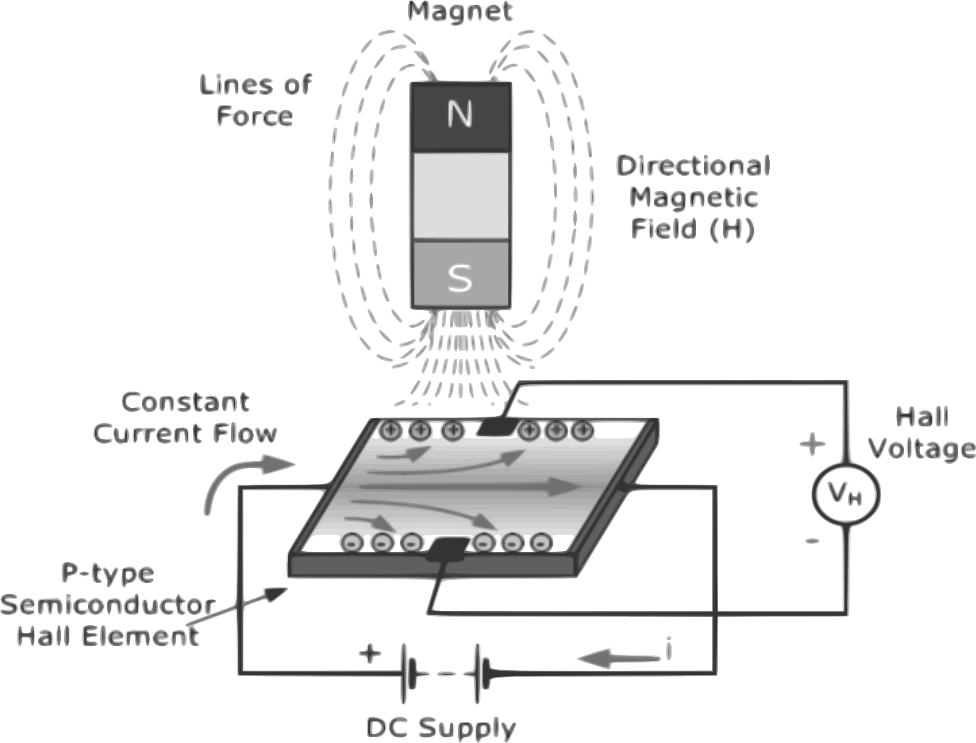
\includegraphics[width=\textwidth]{images/hall_sensor2.png}
	\caption{Block Diagram of an exemplary hall effect sensor. Recreated from \cite{hall_sensor}.} 
	\label{fig:hall_sensor_block}
\end{figure}

\begin{figure}[th]
	\centering
	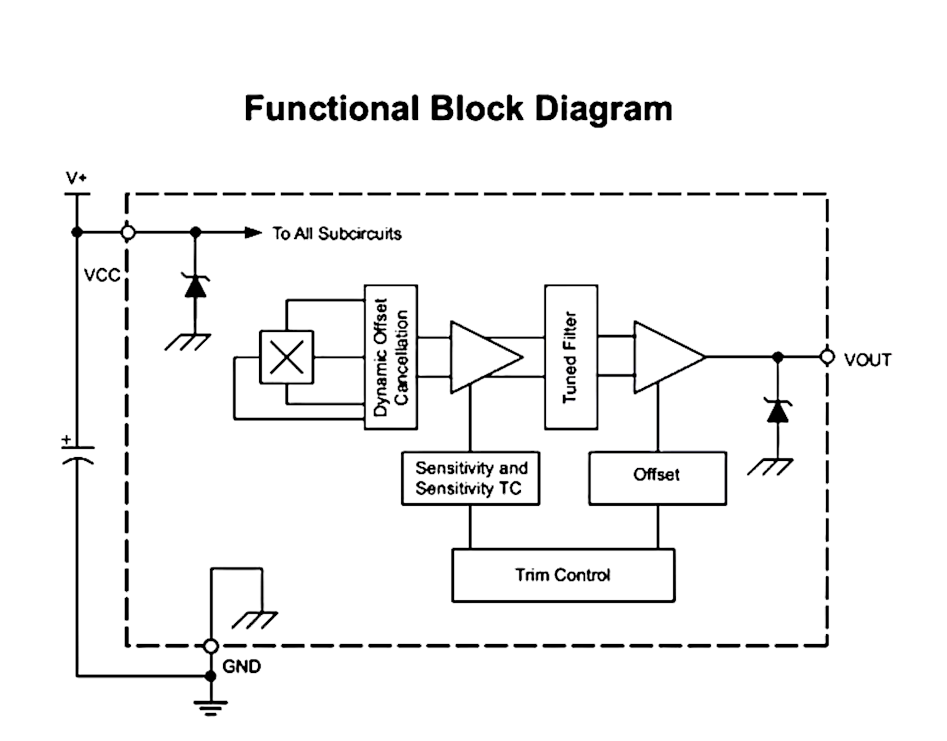
\includegraphics[width=\textwidth]{images/lcs_block_diagram.png}
	\caption{Block Diagram of an exemplary linear current hall effect sensor. The box marked with an X is signifying the hall sensor \cite{hall_effect_element14}.} 
	\label{fig:lcs_block}
\end{figure}

\section{Summary}
The conclusion of this section is, that using an assortment of hall effect sensors, the accurate measurement of flowing current in a live IT environment is very possible. As current through the electric appliance is a direct result of the energy needs of the measured object, the resulting measurement is sufficiently linked to real energy consumption.
Regarding voltage, the exact amount of the quantity is highly dependent on the power quality supplied by the grid. As this factor is mostly independent from the experiment, fluctuations and uncertainties should be reduced by using average measurements over a longer period of time. This can be achieved by evaluating the average of multiple measurements in the order of magnitude of multiple tens or hundred. For this experiment a timing window of 15 minutes is considered as sufficient, and will be chosen as the default measurement interval after averaging.

\pagebreak

\clearpage